%==============================================================================
% Solow Model Cheatsheet - Enhanced Edition
% Exam-Focused Reference for Macroeconomics I
%==============================================================================

\documentclass[a4paper,11pt]{article}

\usepackage{geometry}
\geometry{margin=1in}

\usepackage{amsmath}
\usepackage{amssymb}
\usepackage{mathtools}
\usepackage{graphicx}

\usepackage{xcolor}
\definecolor{blue3}{RGB}{0,0,180}
\definecolor{green3}{RGB}{0,120,0}
\definecolor{orange3}{RGB}{200,100,0}

\usepackage{siunitx}
\sisetup{detect-all}

\usepackage[colorlinks=true,linkcolor=blue3,citecolor=blue3,urlcolor=blue3]{hyperref}

\usepackage{cleveref}

\usepackage{tcolorbox}
\tcbuselibrary{skins,breakable}

\newtcolorbox{derivationbox}[1][]{
    colback=blue!10,
    colframe=blue3,
    coltitle=blue3,
    title={Derivation:},
    fonttitle=\bfseries,
    #1
}

\newtcolorbox{resultbox}[1][]{
    colback=green!10,
    colframe=green3,
    coltitle=green3,
    title={Result Summary:},
    fonttitle=\bfseries,
    #1
}

\newtcolorbox{keyformulabox}[1][]{
    colback=orange!10,
    colframe=orange3,
    coltitle=orange3,
    title={Key Formula:},
    fonttitle=\bfseries,
    #1
}

\usepackage{booktabs}

\usepackage{enumitem}

% Custom commands
\newcommand{\subtitle}[1]{\par\vspace{0.5em}\large\textit{#1}\par\vspace{1em}}
\newcommand{\ktilde}{\tilde{k}}
\newcommand{\ytilde}{\tilde{y}}
\newcommand{\ctilde}{\tilde{c}}

% Title
\title{\textbf{Solow Model Cheatsheet}}
\author{Macroeconomics I - Exam Reference}
\date{}

\begin{document}

\maketitle


\tableofcontents

\clearpage
\pagestyle{plain}

%==============================================================================
\section{Notation and Definitions}
%==============================================================================

\subsection*{Core Variables}
\begin{align*}
& K = \text{capital stock} & L &= \text{labor force} & Y &= \text{output} \\
& A = \text{technology (TFP)} & s &= \text{savings rate} \\
& \delta = \text{depreciation rate} & n &= \text{population growth rate} & g &= \text{technology growth rate}
\end{align*}

\medskip
\subsection*{Per-Worker Variables}
\[
k \equiv \frac{K}{L}, \qquad y \equiv \frac{Y}{L} = f(k)
\]

\medskip
\subsection*{Per-Effective-Worker (Efficiency Unit) Variables}
\[
\ktilde \equiv \frac{K}{AL}, \qquad \ytilde \equiv \frac{Y}{AL} = f(\ktilde)
\]

\medskip
\subsection*{Constant Returns to Scale (CRS)}
\[
F(\lambda K, \lambda L) = \lambda F(K, L) \quad \forall \lambda > 0
\]

\medskip
\subsection*{Fundamental Dynamic Equation}
\begin{align*}
\dot{\ktilde} = s f(\ktilde) - (n + g + \delta) \ktilde
\tag{Dynamic Equation}
\end{align*}

\medskip
\subsection*{Inada Conditions}
\begin{align*}
\lim_{k \to 0} f'(k) = \infty, \qquad \lim_{k \to \infty} f'(k) = 0
\tag{Inada}
\end{align*}

\clearpage

%==============================================================================
\section{Model Setup: Production Function}
%==============================================================================

\subsection*{Aggregate Production}
\begin{align*}
Y = F(K, L) \quad \text{with Constant Returns to Scale}
\tag{Production}
\end{align*}

\subsection*{Capital Accumulation}
\begin{align*}
\dot{K} = sF(K, L) - \delta K
\tag{Capital Accumulation}
\end{align*}

\subsection*{Per-Worker Form}
\begin{align*}
\dot{k} = sf(k) - (n + \delta)k
\tag{Per-Worker Dynamics}
\end{align*}

\subsection*{Per-Effective-Worker Form}
\begin{align*}
\dot{\ktilde} = s f(\ktilde) - (n + g + \delta)\ktilde
\tag{Per-Effective Dynamics}
\end{align*}

\medskip
\begin{tcolorbox}[colback=yellow!10,colframe=yellow!60,title=Break-Even Investment]
The term $(n+g+\delta)\ktilde$ represents \textit{break-even investment}:
\begin{itemize}
    \item $n\ktilde$: capital needed to equip new workers
    \item $g\ktilde$: capital needed for new effective units (technology growth)
    \item $\delta\ktilde$: replacement for depreciated capital
\end{itemize}
\end{tcolorbox}

\clearpage

%==============================================================================
\section{Derivation of Core Results}
%==============================================================================

%-----------------------------------------------------------------------------
\subsection{Derivation 1: Per-Worker Form}
%-----------------------------------------------------------------------------

\begin{derivationbox}
Starting with the capital accumulation equation:
\[
\dot{K} = sF(K,L) - \delta K
\]

Divide both sides by $L$ to get capital per worker:
\[
\frac{\dot{K}}{L} = s \frac{F(K,L)}{L} - \delta \frac{K}{L}
\]

Define $k = K/L$. Using the quotient rule for $\dot{k}$:
\[
\dot{k} = \frac{\dot{K}L - K\dot{L}}{L^2} = \frac{\dot{K}}{L} - \frac{K}{L}\frac{\dot{L}}{L}
\]

Since $\dot{L}/L = n$ (labor grows at rate $n$):
\[
\dot{k} = \frac{\dot{K}}{L} - nk
\]

Substituting $\dot{K}/L = sf(k) - \delta k$:
\[
\dot{k} = sf(k) - \delta k - nk = sf(k) - (n+\delta)k
\]
\end{derivationbox}

\begin{resultbox}
\[
\boxed{\dot{k} = sf(k) - (n + \delta)k}
\]
\end{resultbox}

%-----------------------------------------------------------------------------
\subsection{Derivation 2: Per-Effective-Worker Form}
%-----------------------------------------------------------------------------

\begin{derivationbox}
Starting with $\dot{K} = sF(K,L) - \delta K$

Define effective worker $\ktilde = K/(AL)$ where $A$ grows at rate $g$. Using product rule:
\[
\dot{\ktilde} = \frac{\dot{K}}{AL} - \frac{K}{(AL)^2}(A\dot{L} + \dot{A}L)
\]

Simplify the second term:
\[
\dot{\ktilde} = \frac{\dot{K}}{AL} - \frac{K}{AL}\left(\frac{\dot{L}}{L} + \frac{\dot{A}}{A}\right) = \frac{\dot{K}}{AL} - \ktilde(n+g)
\]

Now $\frac{\dot{K}}{AL} = s\frac{F(K,L)}{AL} - \delta\frac{K}{AL} = s f(\ktilde) - \delta \ktilde$:

\[
\dot{\ktilde} = s f(\ktilde) - \delta \ktilde - \ktilde(n+g) = s f(\ktilde) - (n+g+\delta)\ktilde
\]

Here: $sf(\ktilde)$ is investment, $(n+g)\ktilde$ is dilution from labor and technology growth, $\delta \ktilde$ is depreciation.
\end{derivationbox}

\begin{resultbox}
\[
\boxed{\dot{\ktilde} = sf(\ktilde) - (n + g + \delta)\ktilde}
\]
\end{resultbox}

%-----------------------------------------------------------------------------
\subsection{Derivation 3: Steady-State}
%-----------------------------------------------------------------------------

\begin{derivationbox}
In the steady-state, effective capital per worker is constant:
\[
\dot{\ktilde} = 0
\]

Set the per-effective-worker accumulation equation to zero:
\[
s f(\ktilde^*) - (n+g+\delta)\ktilde^* = 0
\]

Rearrange to solve for steady-state capital:
\[
s f(\ktilde^*) = (n+g+\delta)\ktilde^*
\]

This equilibrium condition states that investment $s f(\ktilde^*)$ exactly equals break-even investment $(n+g+\delta)\ktilde^*$ needed to maintain $\ktilde^*$. At this point, all capital growth goes to replacing depreciated capital and equipping new effective workers.
\end{derivationbox}

\begin{resultbox}
\begin{align*}
\boxed{s f(\ktilde^*) = (n + g + \delta)\ktilde^*}
\tag{SS}
\end{align*}
\end{resultbox}

\medskip
\noindent \textbf{Steady-State Values:}
\begin{align}
\ytilde^* &= f(\ktilde^*) \\
\ctilde^* &= \ytilde^* - (n + g + \delta)\ktilde^*
\end{align}

%-----------------------------------------------------------------------------
\subsection{Derivation 4: Golden Rule}
%-----------------------------------------------------------------------------

\begin{derivationbox}
The steady-state consumption per effective worker is:
\[
\ctilde^* = f(\ktilde^*) - (n+g+\delta)\ktilde^*
\]

Maximize $\ctilde^*$ with respect to $\ktilde^*$ by taking the first-order condition:
\[
\frac{d\ctilde^*}{d\ktilde^*} = f'(\ktilde^*) - (n+g+\delta) = 0
\]

Rearrange:
\[
f'(\ktilde^*_{GR}) = n+g+\delta
\]

The Golden Rule capital $\ktilde^*_{GR}$ equates the marginal product of capital to the required rate of return $(n+g+\delta)$. At this point, the marginal unit of capital produces exactly enough to cover depreciation and population/technology growth, maximizing steady-state consumption.
\end{derivationbox}

\begin{resultbox}
\begin{align*}
\boxed{f'(\ktilde_{GR}) = n + g + \delta}
\tag{GR}
\end{align*}
\end{resultbox}

\clearpage

%==============================================================================
\section{Special Case: Cobb-Douglas}
%==============================================================================

\subsection*{Production Function}

The Cobb-Douglas production function takes the form:
\[
F(K,L) = K^\alpha (AL)^{1-\alpha}
\]

where $\alpha \in (0,1)$ is the capital share of income. The parameter $\alpha$ measures the elasticity of output with respect to capital.

\medskip
\begin{tcolorbox}[colback=blue!5,colframe=blue3,title=Interpretation of $\alpha$]
\begin{itemize}
    \item $\alpha$ = capital share of income (elasticity of output w.r.t. capital)
    \item $1-\alpha$ = labor share of income (elasticity of output w.r.t. labor)
    \item $\alpha$ typically ranges from 0.3 to 0.4 in empirical studies
\end{itemize}
\end{tcolorbox}

\subsection*{Per-Effective Worker Output}

To express output in terms of capital per effective worker $\ktilde = K/(AL)$, we divide the production function by $AL$:

\begin{derivationbox}{Derivation of $f(\ktilde) = \ktilde^\alpha$}
\begin{align}
f(\ktilde) &= \frac{F(K,L)}{AL} \\
&= \frac{K^\alpha (AL)^{1-\alpha}}{AL} \\
&= \left(\frac{K}{AL}\right)^\alpha \\
&= \ktilde^\alpha
\end{align}
\end{derivationbox}

\begin{resultbox}
\begin{align*}
\boxed{f(\ktilde) = \ktilde^\alpha}
\tag{CD-f}
\end{align*}
\end{resultbox}

\subsection*{Marginal Product of Capital}

\begin{derivationbox}{Derivation of MPK}
\begin{align}
f'(\ktilde) &= \frac{d}{d\ktilde} \ktilde^\alpha \\
&= \alpha \ktilde^{\alpha-1}
\end{align}
\end{derivationbox}

\begin{resultbox}
\begin{align*}
\boxed{f'(\ktilde) = \alpha \ktilde^{\alpha-1}}
\tag{CD-MPK}
\end{align*}
\end{resultbox}

Since $\alpha \in (0,1)$, we have $\alpha - 1 < 0$, which implies \textbf{diminishing returns to capital}.

\subsection*{Steady-State Derivation}

\begin{derivationbox}{Derivation of Steady-State Capital}
\begin{align}
s f(\ktilde^*) &= (n+g+\delta)\ktilde^* \\
s(\ktilde^*)^\alpha &= (n+g+\delta)\ktilde^* \\
s\ktilde^{*\alpha-1} &= (n+g+\delta) \\
\ktilde^* &= \left[\frac{s}{n+g+\delta}\right]^{\frac{1}{1-\alpha}}
\end{align}
\end{derivationbox}

\begin{resultbox}
\begin{align*}
\boxed{\ktilde^* = \left[\frac{s}{n + g + \delta}\right]^{\frac{1}{1-\alpha}}}
\tag{CD-SS-k}
\end{align*}
\end{resultbox}

\subparagraph*{Steady-State Output and Consumption}
\begin{align*}
\ytilde^* = \left[\frac{s}{n + g + \delta}\right]^{\frac{\alpha}{1-\alpha}}
\tag{CD-SS-y}
\end{align*}

\begin{align*}
\ctilde^* = \ytilde^* - (n + g + \delta)\ktilde^*
\tag{CD-SS-c}
\end{align*}

\subsection*{Golden Rule Steady State}

\begin{derivationbox}{Derivation of Golden Rule Capital}
\begin{align}
\frac{d\ctilde^*}{d\ktilde} &= 0 \\
\alpha \ktilde^{\alpha-1} - (n+g+\delta) &= 0 \\
\ktilde_{GR}^{\alpha-1} &= \frac{\alpha}{n+g+\delta} \\
\ktilde_{GR} &= \left[\frac{\alpha}{n+g+\delta}\right]^{\frac{1}{1-\alpha}}
\end{align}
\end{derivationbox}

\begin{resultbox}
\begin{align*}
\boxed{\ktilde_{GR} = \left[\frac{\alpha}{n + g + \delta}\right]^{\frac{1}{1-\alpha}}}
\quad
\boxed{s_{GR} = \alpha}
\tag{CD-GR}
\end{align*}
\end{resultbox}

\begin{tcolorbox}[colback=yellow!10,colframe=yellow!60,title=Dynamic Efficiency]
\begin{tabular}{p{0.45\linewidth}p{0.45\linewidth}}
\toprule
\textbf{If $s < s_{GR}$} & \textbf{If $s > s_{GR}$} \\
\midrule
$\ktilde^{*} < \ktilde_{GR}$ & $\ktilde^{*} > \ktilde_{GR}$ \\
$\ctilde^{*} < \ctilde_{GR}$ & $\ctilde^{*} < \ctilde_{GR}$ \\
$f'(\ktilde^{*}) > n+g+\delta$ & $f'(\ktilde^{*}) < n+g+\delta$ \\
Increase $s$ to raise $\ctilde^{*}$ & Decrease $s$ to raise $\ctilde^{*}$ \\
Dynamically efficient & Dynamically inefficient \\
\bottomrule
\end{tabular}
\end{tcolorbox}

\subsection*{Convergence to Steady State}

\begin{derivationbox}{Derivation of Convergence Parameter}
Linearizing around the steady state:
\[
\dot{\ktilde} \approx (1-\alpha)(n+g+\delta)(\ktilde - \ktilde^*)
\]

At the steady state: $sf'(\ktilde^*) = (n+g+\delta)$, so:
\[
\dot{\ktilde} = -(1-\alpha)(n+g+\delta)(\ktilde - \ktilde^*)
\]
\end{derivationbox}

\begin{resultbox}
\begin{align*}
\boxed{\beta = (1-\alpha)(n + g + \delta)}
\tag{CD-Convergence}
\end{align*}
\end{resultbox}

\begin{tcolorbox}[colback=green!5,colframe=green3,title=Properties of $\beta$]
\begin{itemize}
    \item $\beta > 0$ since $0 < \alpha < 1$ and $n+g+\delta > 0$
    \item Higher $\alpha$ $\Rightarrow$ slower convergence
    \item Higher $n$, $g$, or $\delta$ $\Rightarrow$ faster convergence
    \item $s$ does NOT affect convergence speed in Cobb-Douglas
    \item Half-life: $t_{1/2} = \frac{\ln 2}{\beta}$
\end{itemize}
\end{tcolorbox}

\clearpage

%==============================================================================
\section{Dynamic Path, Stability, and Growth}
%==============================================================================

\subsection*{Phase Diagram}

\begin{center}
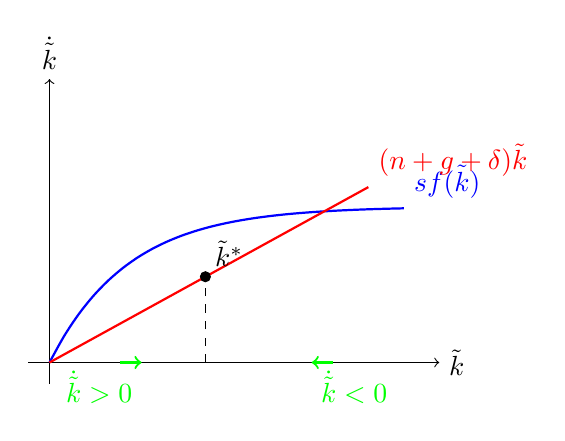
\begin{tikzpicture}[scale=0.9]
    \draw[->] (-0.3,0) -- (5.5,0) node[right] {$\ktilde$};
    \draw[->] (0,-0.3) -- (0,4) node[above] {$\dot{\ktilde}$};
    
    % Investment curve
    \draw[domain=0:5,smooth,variable=\x,blue,thick] plot ({\x},{2.2 * (1 - exp(-0.9*\x))}) node[above right,blue] {$sf(\ktilde)$};
    
    % Depreciation line
    \draw[domain=0:4.5,smooth,variable=\x,red,thick] plot ({\x},{0.55*\x}) node[above right,red] {$(n+g+\delta)\ktilde$};
    
    % Steady state
    \draw[dashed] (2.2,0) -- (2.2,1.21);
    \draw[fill=black] (2.2,1.21) circle (0.07) node[above right] {$\ktilde^{*}$};
    
    % Arrows
    \draw[->,thick,green] (1.0,0) -- (1.3,0);
    \node[green] at (0.7,-0.35) {$\dot{\ktilde} > 0$};
    
    \draw[->,thick,green] (4.0,0) -- (3.7,0);
    \node[green] at (4.3,-0.35) {$\dot{\ktilde} < 0$};
\end{tikzpicture}
\end{center}

\subsection*{Stability Analysis}
\begin{itemize}
    \item \textbf{For $\ktilde < \ktilde^{*}$}: $sf(\ktilde) > (n+g+\delta)\ktilde$ $\Rightarrow$ $\dot{\ktilde} > 0$ (capital accumulates)
    \item \textbf{For $\ktilde > \ktilde^{*}$}: $sf(\ktilde) < (n+g+\delta)\ktilde$ $\Rightarrow$ $\dot{\ktilde} < 0$ (capital depletes)
\end{itemize}

\medskip
\noindent \textbf{Result:} The steady state $\ktilde^{*}$ is \textbf{globally asymptotically stable}.

\subsection*{Transitional Dynamics}
Log-linearization yields:
\[
\gamma_{\ktilde} \equiv \frac{\dot{\ktilde}}{\ktilde} \approx -\beta (\ln \ktilde - \ln \ktilde^{*})
\]

Solution:
\begin{align*}
\ln(\ktilde_t) = (\ln(\ktilde_0) - \ln(\ktilde^{*}))e^{-\beta t} + \ln(\ktilde^{*})
\tag{Transition}
\end{align*}

\subsection*{Conditional Convergence}
The Solow model predicts \textbf{conditional convergence}: an economy grows faster the further it is from its own steady state.

\clearpage

%==============================================================================
\section{Long-Run Growth and Growth Accounting}
%==============================================================================

\subsection*{Long-Run Growth}
In the steady state:
\begin{itemize}
    \item Per-effective variables ($\ktilde, \ytilde, \ctilde$) are constant
    \item Aggregate $Y$ grows at rate $n + g$
    \item Output per worker $y$ grows at rate $g + n$
\end{itemize}

\subsection*{Growth Accounting}
For Cobb-Douglas $Y = K^\alpha (AL)^{1-\alpha}$:
\begin{align*}
g_Y = \alpha g_K + (1-\alpha)(g + n)
\tag{Growth Accounting}
\end{align*}

In steady state: $g_Y = g + n$.

\subsection*{Comparative Statics on Steady State}
\begin{center}
\begin{tabular}{lcc}
\toprule
Parameter & Effect on $\ktilde^{*}$ & Effect on $\ytilde^{*}$ \\
\midrule
$\uparrow s$ (savings) & $\uparrow$ & $\uparrow$ \\
$\uparrow n$ (population growth) & $\downarrow$ & $\downarrow$ \\
$\uparrow g$ (tech growth) & $\downarrow$ & $\downarrow$ \\
$\uparrow \delta$ (depreciation) & $\downarrow$ & $\downarrow$ \\
\bottomrule
\end{tabular}
\end{center}

\clearpage

%==============================================================================
\section{Policy Shocks and Comparative Statics}
%==============================================================================

\subsection*{4-Step Policy Shock Template}

\begin{enumerate}
    \item \textbf{Identify the parameter change:} What parameter changes? ($s$, $n$, $\delta$, $g$)
    
    \item \textbf{Determine new steady state:} Solve with new parameter(s):
    \[
    s' f(\ktilde^{*\prime}) = (n + g + \delta')\ktilde^{*\prime}
    \]
    
    \item \textbf{Compute effects on outputs:}
    \begin{itemize}
        \item $\ytilde^{*} = f(\ktilde^{*})$
        \item $\ctilde^{*} = \ytilde^{*} - (n + g + \delta)\ktilde^{*}$
    \end{itemize}
    
    \item \textbf{Describe transition path:}
    \begin{itemize}
        \item If $\ktilde_0 < \ktilde^{*}_{\text{new}}$: economy accumulates ($\dot{\ktilde} > 0$)
        \item If $\ktilde_0 > \ktilde^{*}_{\text{new}}$: economy decumulates ($\dot{\ktilde} < 0$)
    \end{itemize}
\end{enumerate}

\clearpage

%==============================================================================
\section{Problem-Solving Templates}
%==============================================================================

\subsection*{(a) Derive Steady State and Trajectories}

\begin{enumerate}
    \item Start from fundamental law of motion: $\dot{\ktilde} = s f(\ktilde) - (n + g + \delta)\ktilde$
    \item Set $\dot{\ktilde} = 0$ and solve: $s f(\ktilde^{*}) = (n + g + \delta)\ktilde^{*}$
    \item For trajectories: log-linearize around steady state
    \item Use phase diagram for qualitative analysis
\end{enumerate}

\subsection*{(b) Policy-Change Analysis}

\begin{enumerate}
    \item Identify parameter change ($s \to s'$, $\delta \to \delta'$, etc.)
    \item Find new steady state with new parameters
    \item Compare steady-state values ($\ytilde^{*}, \ctilde^{*}$)
    \item Determine transition direction from initial $\ktilde_0$
\end{enumerate}

\subsection*{(c) Golden Rule with Given $f(\cdot)$}

\begin{enumerate}
    \item Set MPK equal to break-even investment: $f'(\ktilde_{GR}) = n + g + \delta$
    \item Solve for $\ktilde_{GR}$ using the specific $f(\cdot)$ form
    \item Compute $\ctilde_{GR} = f(\ktilde_{GR}) - (n + g + \delta)\ktilde_{GR}$
\end{enumerate}

\subsection*{(d) Per-Effective to Per-Worker Translation}

\begin{enumerate}
    \item Given $A(t) = A_0 e^{gt}$, $L(t) = L_0 e^{nt}$
    \item Per-effective: $\ktilde = K/(AL)$, $\ytilde = Y/(AL) = f(\ktilde)$
    \item Per-worker: $k = K/L = \ktilde \cdot A$, $y = Y/L = \ytilde \cdot A$
    \item In SS: $\ktilde$ constant $\Rightarrow$ $k$ grows at rate $g$, $y$ at $g+n$
\end{enumerate}

\subsection*{(e) Non-Cobb-Douglas Production}

\begin{enumerate}
    \item Identify $f(\ktilde)$ from $F(K, AL)$: $f(\ktilde) = F(\ktilde, 1)$
    \item Apply general SS condition: $s f(\ktilde^{*}) = (n + g + \delta)\ktilde^{*}$
    \item For comparative statics: differentiate implicitly
    \item Verify uniqueness with Inada conditions
\end{enumerate}

\clearpage

%==============================================================================
\section{Common Pitfalls and Tips}
%==============================================================================

\begin{enumerate}
    \item \textbf{Per-effective vs per-worker mix-ups}
    \begin{itemize}
        \item $\ktilde = K/(AL)$ vs $k = K/L$
        \item Dynamic equation: $\dot{\ktilde}$ uses $(n+g+\delta)$, $\dot{k}$ uses $(n+\delta)$
        \item In SS: $\ktilde$ constant, $k$ grows at rate $g$
    \end{itemize}

    \item \textbf{Mistaking steady-state conditions}
    \begin{itemize}
        \item $\dot{k} = 0$ means $k$ is constant (not growing)
        $\dot{\ktilde} = 0$ means $\ktilde$ is constant
    \end{itemize}

    \item \textbf{Misapplying Golden Rule}
    \begin{itemize}
        \item Golden Rule maximizes $\ctilde^{*}$, not $\ytilde^{*}$
        \item Condition: $f'(\ktilde^{*}) = n+g+\delta$
        \item Under CD: $s_{GR} = \alpha$, not $s = 1$
    \end{itemize}

    \item \textbf{Neglecting $A$-growth}
    \begin{itemize}
        \item $g$ affects steady state $\ktilde^{*}$: higher $g$ $\Rightarrow$ lower $\ktilde^{*}$
    \end{itemize}

    \item \textbf{Convergence speed misconceptions}
    \begin{itemize}
        \item $\beta = (1-\alpha)(n+g+\delta)$, NOT $(1-\alpha)$
    \end{itemize}
\end{enumerate}

\clearpage

%==============================================================================
\section{Quick Reference Formulas}
%==============================================================================

\subsection*{Core Variables}
\begin{align*}
\ktilde = \frac{K}{AL}, \quad \ytilde = \frac{Y}{AL} = f(\ktilde) \\
k = \frac{K}{L}, \quad y = \frac{Y}{L} = f(k)
\end{align*}

\subsection*{Dynamic Equations}
\begin{align*}
\dot{\ktilde} &= s f(\ktilde) - (n+g+\delta)\ktilde \\
\dot{k} &= s f(k) - (n+\delta)k
\end{align*}

\subsection*{Steady State}
\begin{align*}
s f(\ktilde^{*}) &= (n+g+\delta)\ktilde^{*} \\
\ytilde^{*} &= f(\ktilde^{*}) \\
\ctilde^{*} &= \ytilde^{*} - (n+g+\delta)\ktilde^{*}
\end{align*}

\subsection*{Cobb-Douglas ($f(\ktilde) = \ktilde^\alpha$, $0 < \alpha < 1$)}
\begin{align*}
\ktilde^{*} &= \left[\frac{s}{n+g+\delta}\right]^{\frac{1}{1-\alpha}} \\
\ytilde^{*} &= \left[\frac{s}{n+g+\delta}\right]^{\frac{\alpha}{1-\alpha}} \\
\ktilde_{GR} &= \left[\frac{\alpha}{n+g+\delta}\right]^{\frac{1}{1-\alpha}} \\
s_{GR} &= \alpha
\end{align*}

\subsection*{Growth Rates in SS}
\begin{itemize}
    \item Per-effective ($\ktilde, \ytilde, \ctilde$): constant ($0$ growth)
    \item $k$ grows at rate $g$
    \item $y$ grows at rate $g+n$
    \item $Y$ grows at rate $g+n$
\end{itemize}

\subsection*{Convergence}
\[
\beta = (1-\alpha)(n+g+\delta), \quad 
\ln(\ktilde_t) = (\ln(\ktilde_0) - \ln(\ktilde^{*}))e^{-\beta t} + \ln(\ktilde^{*})
\]

\subsection*{Growth Accounting}
\[
g_Y = \alpha g_K + (1-\alpha)(g+n)
\]

\clearpage

%==============================================================================
\section{Implementation Notes}
%==============================================================================

\subsection*{Changes from Original Version}

\begin{enumerate}
    \item \textbf{Enhanced Preamble}: Added tcolorbox, siunitx, cleveref, and hyperref packages with proper configuration
    \item \textbf{Derivation Boxes}: Created dedicated derivation environments (derivationbox, resultbox) using tcolorbox for clear visual separation
    \item \textbf{Narrative Derivations}: Added step-by-step derivations with inline commentary for:
        \begin{itemize}
            \item Per-worker to per-effective transformation
            \item Steady-state derivation
            \item Golden Rule derivation
            \item Cobb-Douglas closed forms
            \item Convergence speed
        \end{itemize}
    \item \textbf{Equation Numbering}: Used \texttt{\ tag{}} for consistent equation references
    \item \textbf{Visual Hierarchy}: Added colored boxes for key interpretations and properties
    \item \textbf{Consistent Notation}: Used $\ktilde$, $\ytilde$, $\ctilde$ commands throughout
\end{enumerate}

\subsection*{Packages Used}
\begin{itemize}
    \item amsmath, amssymb, mathtools: Mathematics
    \item graphicx: Graphics
    \item xcolor: Color support
    \item siunitx: Units and number formatting
    \item cleveref: Smart cross-references
    \item hyperref: Hyperlinks
    \item tcolorbox: Colored boxes for derivations
    \item booktabs: Publication-quality tables
\end{itemize}

\subsection*{Compilation}
Compile with: \texttt{pdflatex} or \texttt{lualatex}

\clearpage

\end{document}